

\setlength{\abovedisplayskip}{3pt}
\setlength{\belowdisplayskip}{3pt}
\setlength{\abovedisplayshortskip}{3pt}
\setlength{\belowdisplayshortskip}{3pt}

	\thispagestyle{empty}
	\rule{\linewidth}{1pt}
	
	\vspace{6pt}				%Die Leerzeilen müssen tatsächlich da sein, sonst funktioniert das nicht
	
	\begin{minipage}{0.6\textwidth}
		\begin{flushleft} 
		\Profs
		\end{flushleft}
	\end{minipage}
	\begin{minipage}{0.39\textwidth}
		\begin{flushright}
			Universität Hamburg
		\end{flushright}
	\end{minipage}

	\rule{\linewidth}{1pt}\\
	\begin{center}
		\Large{\textsf{\titel}}\\
		\small\textsf{Version vom \today}
\vspace{8pt}
\end{center}


\begin{figure}[htbp]
    \centering
    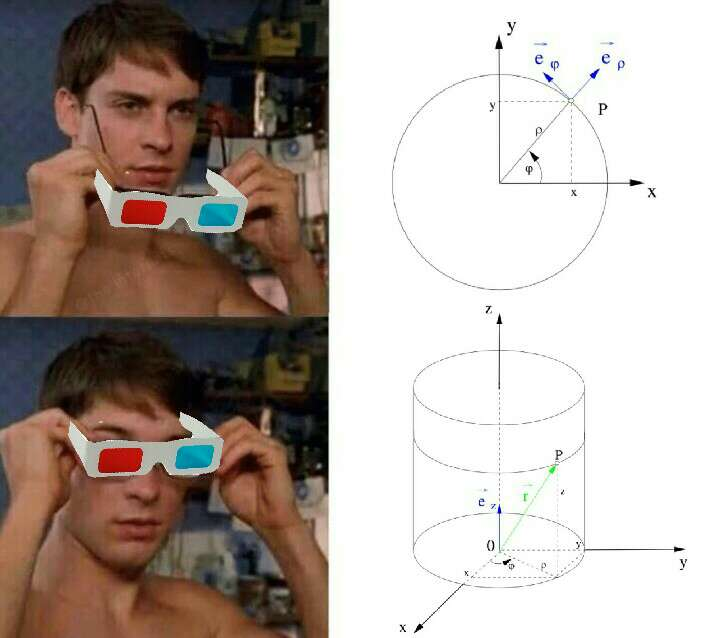
\includegraphics[width=.55\textwidth]{Dateien/3D_Analysis.jpg}\\
    Analysis, aber diesmal in 3D!\\
\end{figure}
\vfill
Grüßt euch, dies sind die Community MfP3-Notizen. \\

Sissi und ich erstellen sie als Nachbereitung der Vorlesung und sie dienen als eine schnelle Quelle von Definitionen und einfachen Beispielen (um sich einen Überblick zu verschaffen), wichtigen Bemerkungen aus den Übungen, sowohl als Klausurnotizen. Wir bewundern die informellen Notizen zum MfP1- und MfP2-Tutorium von Robin Löwenberg und Fabian Balzer und haben uns entschloßen mit dem gleichen Stil weiterzumachen, da es keine MfP3 und MfP4 Tutoriumnotizen mehr gibt. Die Templates wurden von Fabian erstellt und sind auf seiner Github-Seite verfügbar:  \url{https://github.com/Fabian-Balzer/MfP2-Notizen}. Zusätzlich benutzen wir das Lehrwerk Mathematik von Tilo Arens als eine Quelle von guten Beispielen. Das Buch können wir jedem empfehlen, der auch Giancoli mag und am besten an Beispielen lernt. Bei Anmerkungen oder Fragen schreibt uns einfach auf Whatsapp, Discord oder GitHub an. \\ 

Möge die Macht der endlosen zerbrochenen Kreiden mit euch sein :)

\cfoot{\pagemark}
